\chapter{Review of relevant literature} \label{cha:Literature-review}

\section{Introduction} \label{sec:Lit-Review-Introduction}

There are two major fields of literature relevant to this project: firstly, studies and technical reports delivered within engineering organisations relating to real spacecraft missions. Secondly, there has been a long history of theoretical study into optimising spacecraft trajectories, from early impulsive spacecraft research to more recent low-thrust scenarios.

% -------------------------------------------------------- Past missions --------------------------------------------------------
\section{Past missions} \label{sec:Past-missions}

% include review of \cite{Schoenmaekers2004} Post launch optimisation of SMART-1

While \textcite{LePage1991} shows that there have been numerous Earth-orbiting satellites using electric thrusters for attitude control or station keeping, only a small number of spacecraft have ever escaped the Earth's sphere of influence using electric propulsion as the primary thrust. These are listed in \autoref{tab:Past-low-thrust-missions}, along with key specifications of their respective propulsion systems. Thrust is the maximum force that the primary propulsion system can exert on the craft. Power consumption is the amount of electrical power used to operate at this maximum thrust. Specific impulse, $I_{sp}$, is the momentum added by the thrusters per unit weight-on-Earth of propellant, and consequently represents the fuel efficiency of the thrusters. Electric propulsion is characterised by relatively high $I_{sp}$.

\begin{table}[ht]
  \caption{Past low-thrust missions to escape Earth's sphere of influence}
  \label{tab:Past-low-thrust-missions}
    \begin{center}
    \begin{minipage}{\textwidth}
    \begin{tabular}{C{0.2\textwidth} C{0.25\textwidth} C{0.2\textwidth} C{0.1\textwidth} c}\toprule
      Spacecraft & Propulsion type & Total Power \linebreak Consumption \linebreak (W) & Total Thrust \linebreak (mN) & $I_{sp}$ (s)\\\midrule
      DS-1\footnote{\textcite{web_DS-1}} & Electrostatic Ion Thruster & 2100 & 92 & 3300\\
      Hayabusa\footnote{\textcite{web_Hayabusa}} & $4\times$ Microwave ECR Thrusters & 1400 & 32 & 3200\\
      SMART-1\footnote{\textcite{web_SMART-1}} & Hall Effect Thruster & 1200 & 73 & 1640\\
      Dawn\footnote{\textcite{web_Dawn}} & Electrostatic Ion Thruster & 2100 & 90 & 3100\\\midrule
      Lunar Mission BW-1\footnote{\textcite{web_BW-1}} & $4\times$ Pulsed Plasma Thrusters & 220 & 4.9 & 2753\\
      & Thermal Arcjet & 801 & 103 & 486 \\\bottomrule
    \end{tabular}
    \end{minipage}
    \end{center}
\end{table}

For the purposes of comparison, the Apollo program trans-lunar injection (TLI) was performed using a chemical propulsion system providing a thrust of approximately 1~MN (9 orders of magnitude greater than \BW) on a mass of 119,900~kg (only 3 orders of magnitude greater than \BW) at a specific impulse of 421~s. The Saturn V third stage that performed the TLI is shown at launch in \autoref{fig:SaturnV}.

\begin{figure}[ht]
  \begin{center}
  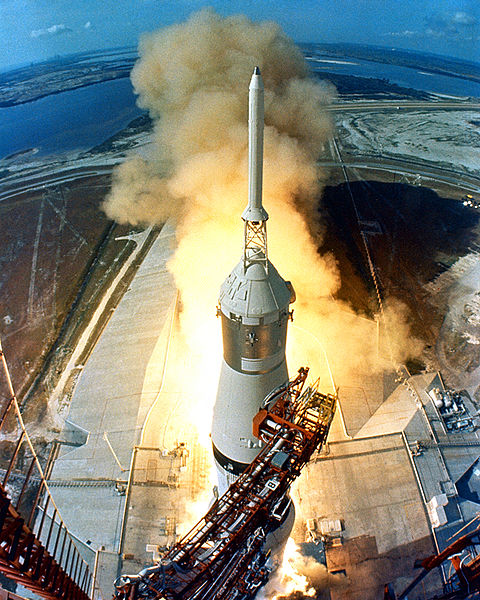
\includegraphics  [width=0.7\textwidth] {Images/Apollo_11_Launch2.jpg}
  \end{center}
  \caption{Saturn V from the Apollo program. Image used courtesy of NASA.}
  \label{fig:SaturnV}
\end{figure}

\subsection{Deep Space One}
Deep Space One (DS-1), shown conceptually in \autoref{fig:DS-1}, was launched on 24 October 1998 with a mass of 374~kg \parencite{web_DS-1}. After launch, an electrostatic ion thruster took over propulsion on its one-way mission to the asteroid 9969~Braille and the comet 19P/Borrelly. This thruster generated 92~mN of thrust at a maximum input power of 2100~W. DS-1 had several similarities to the intended mission of \BW.

\begin{figure}[ht]
  \begin{center}
  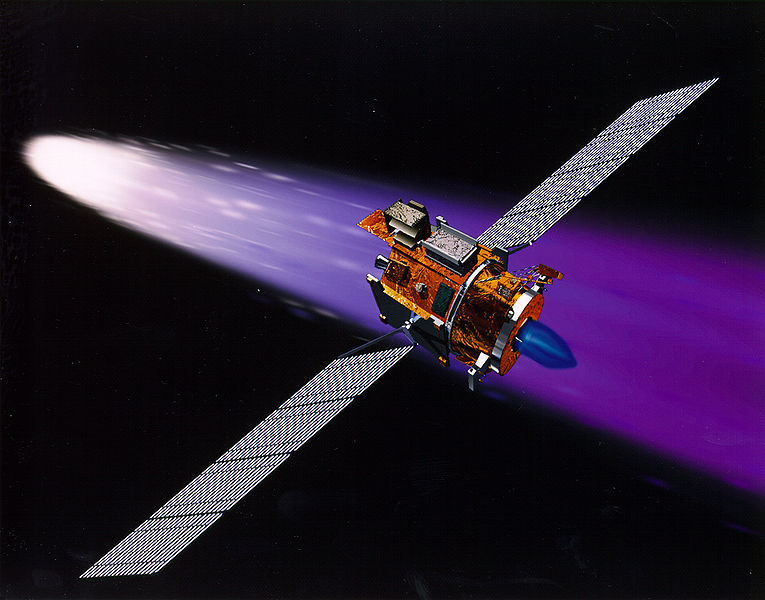
\includegraphics [width=0.7\textwidth] {Images/765px-Deep_Space_1_using_its_ion_engine.jpg}
  \end{center}
  \caption{Deep Space One. Image used courtesy of NASA.}
  \label{fig:DS-1}
\end{figure}
 
\textcite{Rayman1997} state that once or twice each week the spacecraft had to rotate away from its thrust vector in order to collect optical navigation pictures and communicate with the Deep Space Network (DSN) on Earth, which required shutting down the propulsion system. Key differences from \BW\ however, include the frequency and duration of these thrusting and coasting phases, and the nature of the trajectory. The interplanetary trajectory of DS-1 was dominated by a heliocentric orbit, with perturbations from the Earth, Mars and a number of asteroids. This means that the thrust vector was almost tangential to the orbital velocity around the Sun, and therefore the optimal orientation of solar panels (towards the Sun) was always perpendicular to the desired thrust vector (around the Sun). In contrast to this, \BW\ will occupy a cis-lunar orbit. This poses two difficulties: not only will the trajectory optimisation have to switch its reference frame from Earth-centric to lunar-centric in mid-flight, but optimal orientation of the solar panels relative to the direction of thrust is constantly changing. To overcome this the thrusting profile of \BW\ must shut down much more frequently than DS-1 did: hourly, rather than weekly, so that it can point its solar panels towards the Sun to recharge.

\subsection{Hayabusa}
Hayabusa (launched 9 May 2003), shown conceptually in \autoref{fig:Hayabusa}, was designed by the Japanese Aerospace Exploration Agency (JAXA) to perform a rendesvouz with asteroid 25143~Itokawa \parencite{web_Hayabusa}. It had a launch mass of 510~kg, including 130~kg of xenon gas used by the four microwave ECR (Electron Cyclotron Resonance) thrusters, providing 4$\times$8~mN = 32~mN thrust at maximum input power of 4$\times$350~W = 1400~W. Hayabusa had a similarly weak thrust to \BW, but was once again in a heliocentric orbit. Hayabusa successfully re-entered Earth's atmosphere and was recovered near Woomera, South Australia in June 2010, despite numerous failures including almost complete failure of all four ECR thrusters.

\begin{figure}[ht]
  \begin{center}
  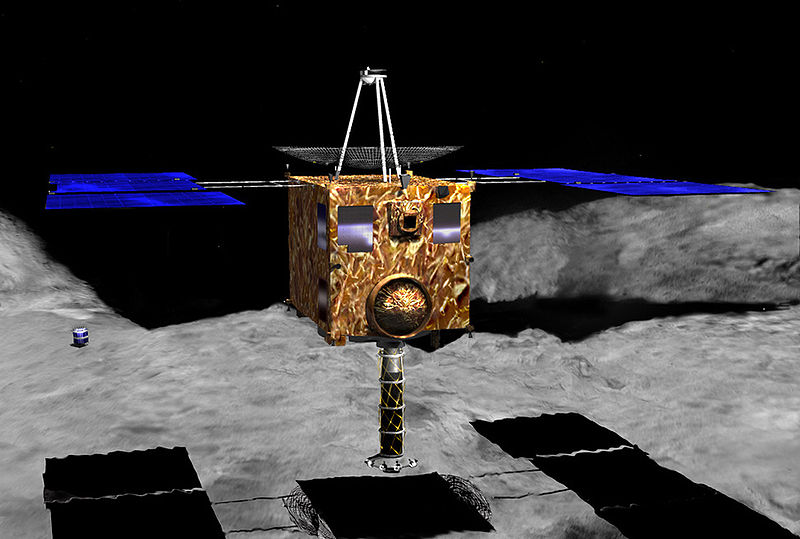
\includegraphics [width=0.7\textwidth] {Images/800px-Hayabusa_hover.jpg}
  \end{center}
  \caption{Japanese Hayabusa probe. Image used courtesy of J. Garry.}
  \label{fig:Hayabusa}
\end{figure}

\subsection{SMART-1}
Small Missions for Advanced Research in Technology One (SMART-1) (launched 27 September 2003) had a Hall effect plasma thruster providing 73~mN thrust at 1200~W power consumption \parencite{web_SMART-1}. The craft, shown conceptually in \autoref{fig:SMART-1}, was a comparable size to \BW, but twice as heavy: 367~kg including 80~kg of xenon propellant. On September 3, 2006 SMART-1 was deliberately crashed into the Moon's surface. This mission profile is closest to that intended for \BW, but had an order of magnitude higher thrust.

\begin{figure}[ht]
  \begin{center}
  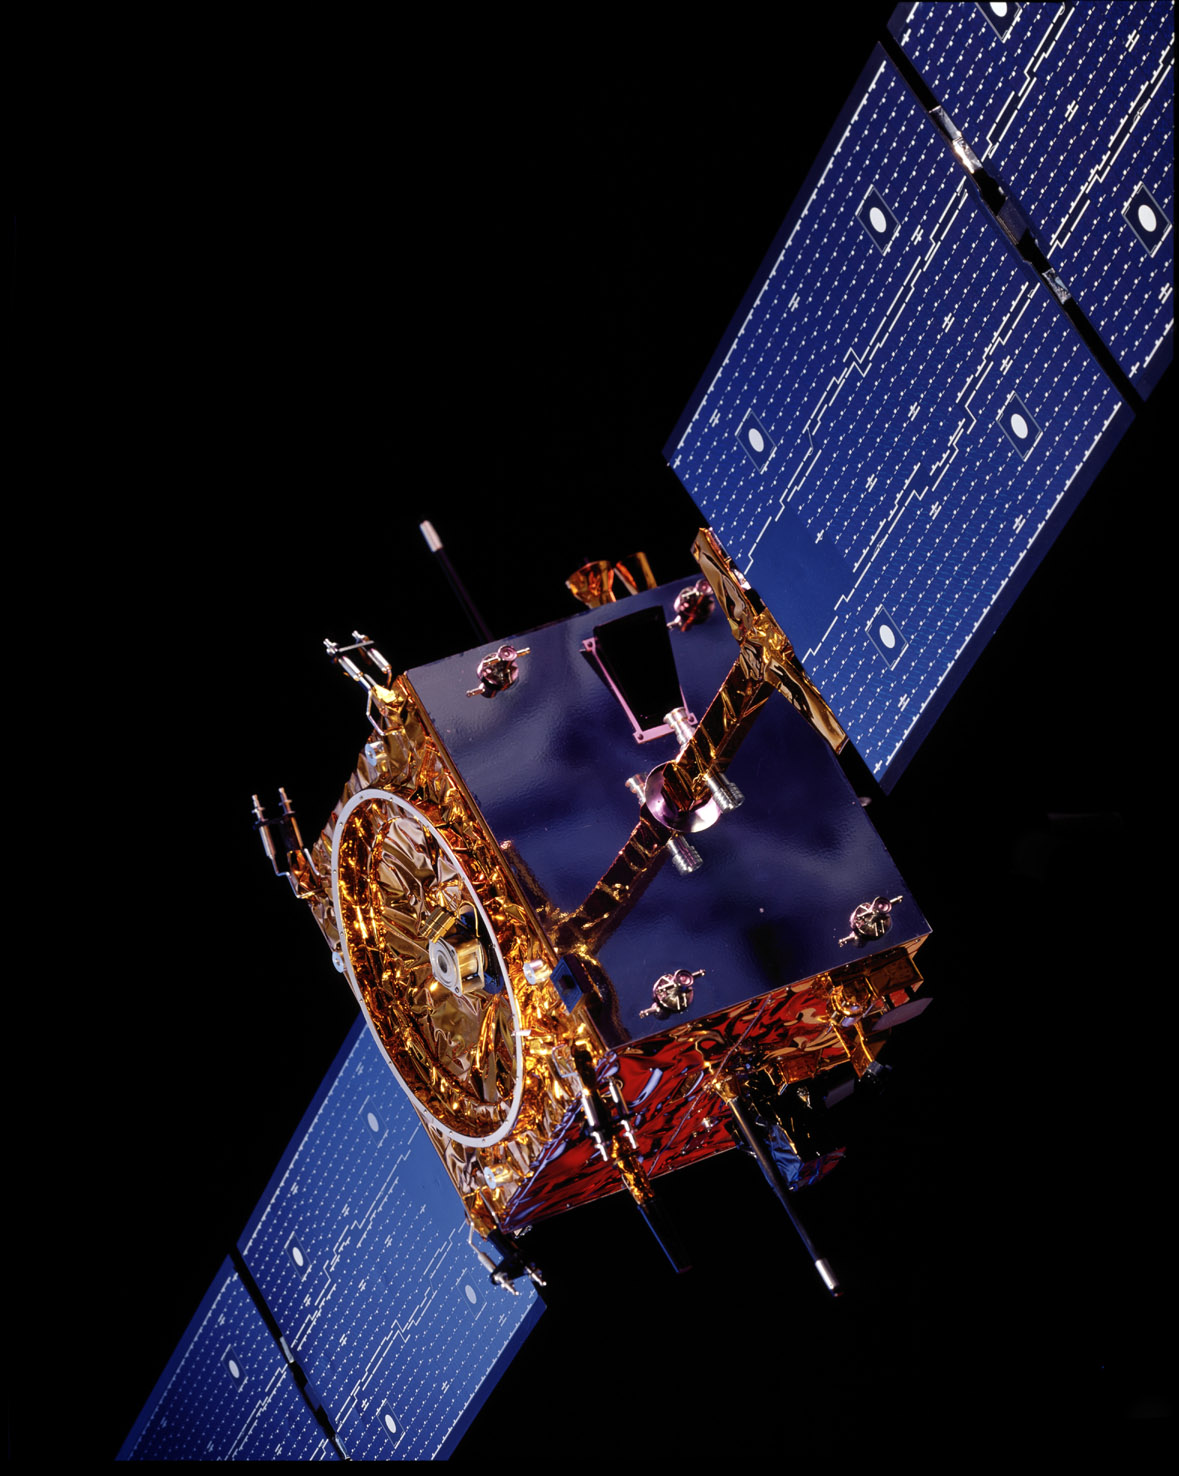
\includegraphics [angle=90,width=0.7\textwidth] {Images/SMART-1.jpg}
  \end{center}
  \caption{SMART-1. Image used courtesy of USGS.}
  \label{fig:SMART-1}
\end{figure}

\subsection{Dawn}
Dawn (launched 27 September 2007) is using the same thrusters developed for DS-1 to propel it towards the dwarf planet 1~Ceres by 2015 \parencite{web_Dawn}, following a successful rendezvous with the main-belt asteroid 4~Vesta in June 2011. Getting to Vesta it consumed 275~kg xenon, and will use another estimated 110~kg to get to Ceres, out of a total of 425~kg of on-board propellant. Dawn, shown conceptually in \autoref{fig:Dawn}, had a total launch mass of 1250~kg.

\begin{figure}[ht]
  \begin{center}
  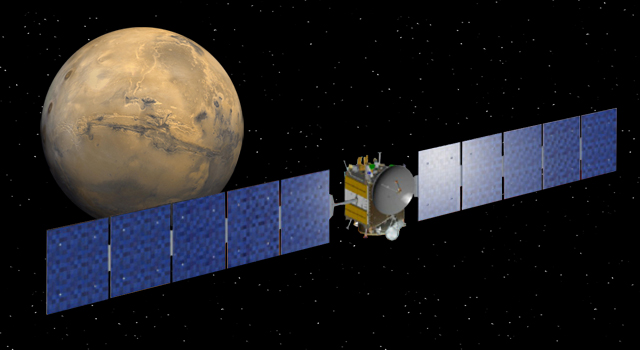
\includegraphics  [width=0.7\textwidth] {Images/mars-browse.jpg}
  \end{center}
  \caption{Dawn. Image used courtesy of NASA.}
  \label{fig:Dawn}
\end{figure}

\subsection{Planned missions}
Planned electrically propelled missions include SMART-2, also known as LISA Pathfinder \parencite{web_SMART-2}, and Space-Technology 7 (ST-7) to be launched by NASA. Common to all of these missions is thrust substantially higher than \BW\ will have available, and consequently \BW\ will have a less flexible escape trajectory.

\BW\ will be only the fifth electrically propelled spacecraft to leave Earth orbit, and the first mission with this type of electric propulsion.



% -------------------------------------------------------- Optimisation methods --------------------------------------------------------

% \cite{McKay2011} provide a survey of non-keplerian orbits, which they define as any orbit with forces additional to the primary point-mass gravitational force. Their study was focussed towards using low thrust propulsion to maintain a stable orbit in the presence of these secondary forces, and while \BW1 requires a transfer trajectory rather than a stable orbit their paper does conclude that there are some serious deficiencies with established research in the area: \enquote{It is clear, however, that work still has to be done to transform the steadily growing body of literature on highly-non-Keplerian orbits from interesting theory into actual, practical missions.}
%evolutionary algorithms often need distributed computing environments due to the number of computations involved \textcite{Lee2005}
%genetic algorithms and simulated annealing \textcite{Lee2005}
%Pareto-optimality based on the economic theory by Italian Vilfredo Pareto, implying that it is the best solution that can be found without compromising other objectives, in this case the best fuel efficiency that can be found without taking an unreasonable amount of time. \parencite{Lee2005, Coverstone2000}
%\textcite{Enright1992} hermite simpson/RK integration, direct shooting/multiple shooting/collocation, concludes -- direct transcription, NLP, \enquote{parallel shooting} RK
%\begin{enumerate}
%\item future work - lower thrust levels, lower initial and final orbits, non-coplanar transfers
%\item size of problem - much better mesh distribution, exploit sparsity
%\item lunar eccentricity and better geopotential do not affect problem size (just time to solve; longer computation each step, but doesn't increase the number of steps).
%\end{enumerate}
%Pierson \& Kluever optimised Earth escape, backwards propagation for Moon \enquote{capture} to maximise lunar energy after a given time, with a cruise phase in between.
%Comparison of retrograde and posigrade terminal orbits. Posigrade gives better performance.
%Very minimal improvement on initial guess suggests optimisation method ineffective.
%\enquote{Hybrid} direct/indirect approach.
%100,000~kg and 2942~N. What kind of electric propulsion?! And are they suggesting sending the ISS to lunar orbit?!
%Uses SQP to solve 2PBVP
%Melbourne and Sauer - Mars trajectories under solar gravity only
%Breakwell and Rauch - patched two-body trajectories
%Not much work on reduced three-body problem
%London and Stuhlinger - patched two-body segments
%Golan and Breakwell - variable thrust magnitude trajectories with no coasting arcs
%Enright and conway - collocation, determining a single minimum fuel, low thrust, earth-moon transfer.
%\textcite{Kluever1996} outlines his experimental procedure to find an initial guess: simulate under thrust, modifying phase time until near SOI. Then simulate for 7-8 days to observe the lunar fly-by, adjusting initial angle (in a 2D moon-fixed frame) until coasting trajectory enters SOI with negative moon-relative radial velocity component. Backwards propagate the lunar descent, adjusting phase length until the orbital energy is about the same as the end of the coasting arc.
%Citing other peoples' graphs in Lit Review: .... Reproduced from \cite{}
%\textcite{Kluever1997} extends the work to 3D, even includes a polar lunar orbit. Still starting from very high earth orbit, still much higher thrust. Uses direct optimisation but pontryagin necessary conditions to parameterise the intial guess control profile.
%Initial guess based on 2D optimisations for GEO-HLO. Optimisation slowly converts plane change from HLO-LLO phase  until it is almost entirely included in GEO-HLO phase.
%T/W ratio of 1.3e-4
%\textcite{Kluever1995} assumes initial LEO in lunar plane.
% All constant thrust, constant mass flow, giant spacecraft, does not address initial launch (inclination, capability to launch that mass). Due to simplifications like no external forces and constant thrust, the inverse costate equations were found allowing the Pontryagin principle to be exploited in order to get a very accurate initial guess for the thrust profiles in ascent and descent phases. SQP is then used to blend the phases together.
% \cite{Herman1998}

\section{Optimisation methods} \label{sec:Optimisation-methods}
Traditional high-thrust chemical rocket trajectories do not need optimisation for lunar missions, since the duration is sufficiently small that perturbing forces are negligible. In the resulting restricted three-body scenario (the Earth and Moon are static, with a spacecraft of negligible mass orbiting them) there are simple analytical solutions for the trajectory.

As outlined in \autoref{cha:Objectives} the task of optimising a low-thrust trajectory is somewhat more complex due to the long duration of forces acting on the orbit requiring lengthy integrations. For the reader unfamiliar with optimisation, an outline is provided in \autoref{cha:Optimisation}. Specific trajectory optimisation techniques available to accomplish this task are described in \autoref{sec:Techniques}. This section addresses how effective previous studies have found those methods to be.

% Optimal control
\subsection{Optimal control} \label{sub:Optimal-control-lit}

\textcite{Golan1994} performed some of the earliest trajectory optimisation for low-thrust spacecraft, based on optimal control laws. Their study assumed a specific thrust of $9.81\times10^{-3}\text{ ms}^{-2}$, over 200 times more thrust per kilogram than \BW\ will have. While their trajectory analysis does allow for a variable thrust engine, it does not consider practical issues such as coasting phases to recharge the batteries, or transitions through the Earth's shadow. The larger thrust allows a much shorter transfer time than anticipated for \BW, so weaker perturbations such as the Earth's oblateness and the gravitational pull of the Sun and Jupiter were neglected.

\textcite{Guelman1995} performed a similar optimal control based trajectory analysis within a three-body plane. An interesting difference to \citeauthor{Golan1994}'s approach is that \citeauthor{Guelman1995} centred his coordinate system at the Earth-Moon barycentre. This smoothes the equations of motion in the region where the Earth and Moon have comparable influence on the spacecraft; however, since a lunar transfer generally spends very little time in this region, it is usually preferable to model with the conceptually easier Earth- and lunar-centred frames.
 
\citeauthor{Guelman1995} still uses a very simplified gravitational model, with a continuously thrusting spacecraft. Variable thrust is allowed for by minimising the total thrust required to achieve a lunar orbit/impact given a constant thrust duration. While this approach achieved lower magnitude thrust profiles than \citeauthor{Golan1994} (for 1000 hours of thrust \citeauthor{Guelman1995} found a maximum of $4.3\times10^{-3}\text{ ms}^{-2}$ was required), it is inappropriate in the current scenario since the mission is constrained by specific impulse (total thrust delivered over the flight) rather than thrust duration. Furthermore, calculating the gravitational field within a barycentric frame becomes increasingly complex with the number of bodies in the gravitational model, making it unsuitable for very low thrust missions which must allow for the weaker perturbations mentioned above.

% need review of \cite{Guelman2000}

\textcite{Pierson1994} developed a three stage approach to solving optimal planar Earth-Moon trajectories. The three stages consisted of a constant thrust Earth-escape, a cis-lunar coast, and a constant thrust lunar capture. This method was extended to a full three-dimensional problem by \textcite{Kluever1995,Kluever1996,Kluever1997}. However, all of these papers assume a continuous thrust profile which is incompatible with both \BW's thrust constraints, and the inherent restrictions placed on thrusting by passing through the Earth's shadow. Furthermore, the optimisation method developed in these papers is adapted from \textcite{Edelbaum1964}, using curve fitting to develop an approximate solution with much less computational effort than the analytical methods utilised previously.

\subsection{Nonlinear programming} \label{sub:NLP-lit}

% This is indicative of increasing levels of non-linearity leading to numerical techniques.
% \cite{Herman1998} parallel Runge-Kutta method optimal Earth-Moon transfers (with continuous thrust? without shadowing?)
% \cite{Enright1992} collocation method - optimal?

\textcite{Betts1993} investigated numerical techniques to determine near-optimal trajectories. In particular, they utilised direct transcription and collocation to approximate the optimisation problem, which was then solved numerically using sparse nonlinear programming.
 
\textcite{Betts1994} introduced a package called Sparse Optimal Control Software (SOCS), and concluded that it is a very computationally efficient method for numerically optimising low-thrust trajectories that include non-linearities caused by perturbing forces. This appears to be a very promising approach, but \textcite{Betts2000} acknowledges that none of these papers included tesseral harmonics of the Earth's gravitational field, third-body gravitational perturbations from the Sun, Moon, or Jupiter, variable thruster duty cycles, the Earth's shadow limits, or atmospheric drag at low altitudes. These papers all used an orbit-to-orbit transfer, with a spacecraft thrusting
 at $1.25\times10^{-4}\text{ ms}^{-2}$ as a test case (this is still an order of magnitude greater thrust than \BW).

The direct transcription approach of \textcite{Betts1993} was extended by \textcite{Erb_thesis} and then \textcite{Betts2003}, by optimising a lunar transfer from GTO employing solar electric propulsion; a mission profile very similar to that of SMART-1. These papers verified that the direct transcription method with sparse non-linear programming is a suitable approach for low-thrust lunar missions, but once again assumed constant thrust throughout the transfer, ignoring Earth shadowing, as well as neglecting tesseral Earth harmonics. While this method may be useful for optimising \BW, as a numerical approach it is not guaranteed to find the optimal path. The performance is also heavily reliant on the initial guess, as highlighted by \textcite{Betts2003}: 

\begin{quotation}The design of an initial guess for a trajectory with a vast number of revolutions, significant inclination changes, capturing and orbital corrections is a challenging task on its own.\end{quotation}

\textcite{Letterio_thesis} described the optimisation of a low thrust transfer using an identical thrust regime to \BW\ (in fact, \citeauthor{Letterio_thesis}'s study was completed as part of the same project with Universit\"{a}t Stuttgart). However, this study only covers the ascent phase, from geosynchronous transfer orbit (GTO) to the outer limits of the van Allen belts, using the higher thrust arcjet. The emphasis was on increasing the radius of the orbit as quickly as possible to escape the van Allen belts. Furthermore, at these relatively low altitudes the gravitational perturbations due to the Moon's gravity are fairly uniform. This limits the extent to which they can be exploited to optimise the trajectory of the spacecraft.

An interesting series of articles in \emph{Acta Astronautica} describe a competition devised by ESA to develop a benchmark test for low thrust optimisation. As the winners of the inaugural competition, held in 2007, \textcite{Petropoulos2007} summarised their findings: 

\begin{quotation}...it seems that a rough global search, based on simple numerical schemes coupled with mission design intuitions, is a necessary precursor activity to the local optimisation, and one which is a rich area for research.\end{quotation}

The 2007 competition was dominated by gravity assists to maximise a spacecraft's velocity, and as such is most relevant to inter-planetary low-thrust trajectories. Several entries attempted to optimise direct transfers from Earth to the target orbit, a scenario with similarities to the planned lunar transfer of \BW. In particular, \textcite{Dachwald2007} developed a program that combines evolutionary algorithms and neural networks to search for an optimal thrust profile. Despite the apparent failure of this method in the competition, their diagnosis of the resulting trajectory demonstrates key aspects of exploiting gravitational perturbations. Due to the short timescale of the competition this research was not continued.

\subsection{Gradient projection methods}\label{sub:Gradient-methods-lit}
\subsection{Sequential quadratic programming} \label{sub:SQP-lit}
\subsection{Other methods} \label{sub:Other-lit}

There are of course many alternatives to gradient based methods of optimisation. Techniques such as genetic algorithms and simulated annealing have attracted an increasing amount of interest in recent decades, as outlined by \textcite{Ren2007}. The primary advantage of these methods is that they provide a better global search before descending into a basin of convergence. Unfortunately there is still no way to be certain that the basin selected will have a better optimum than others, however an implicit assumption that the gradient is generally fairly uniform across the search area (that is, the problem is not very stiff) suggests that the basin with a better objective function at the top will have a better objective function at the bottom also. The assumption of a non-stiff search area also implies that the optimal solution will be located at the bottom of the widest basin of convergence, which is additionally the most likely to be found by the search algorithm.

%Ravines in the search area
% Particularly since change the starting conditions - eg. launch window - by a little bit and the cumulative effect of lunar gravity is hugely different at the end (Chaos theory). However, change it by eg. a month and the Moon is back in the same place.

Reviewed literature such as \textcite{Dachwald2005} and \textcite{Jackson2008} has shown an increasing trend for these methods to be used in trajectory optimisation, albeit often for a global search combined with a gradient-based method to find the local optimum within the basin of convergence. 

An interesting methodological approach to optimisation is presented by \textcite{Jackson2008}. Rather than developing an analytic equation to optimise, or a numerical algorithm to iteratively determine a search direction, a coarse mesh of possible trajectories is plotted based on a few controlled parameters. The largest basin of convergence is then selected based on the assumption that it will be the most robust - even if the global optimum is found using another technique, the spacecraft will never be able to follow that trajectory \emph{exactly}. If the basin of convergence is too narrow, any number of unexpected events could easily push the spacecraft onto a severely sub-optimal trajectory, potentially resulting in the spacecraft not completing its mission. Iteratively calculating trajectories over a mesh of possible launch parameters determines a near-optimal trajectory, within a very broad basin of convergence. While the test case used by \textcite{Jackson2008} involved continual thrust from Earth orbit to the Sun-Earth libration point L1, the methodological nature of this approach allows easy implementation of discontinuous thrust profiles for \BW. This will allow experimentation with exploiting lunar gravitational assists, as well as multiple non-linearities ignored or neglected in previous studies.

%\enquote{According to these classifications, the sequential gradient restoration algorithm (SGRA \parencite{Miele1975}) is an indirect method as are the codes ASTROP developed by Biggs et al. (19XX) and BNDSCO \parencite{Burlisch1971}. ASTROP has been used at the European Space Operations Center (ESOC) extensively for exo-atmospheric trajectory optimization. POST \parencite{Brauer1987} uses a single shooting direct method with control parametrization; it has been developed by US industry. OTIS \parencite{Hargraves} uses a direct collocation method and has been developed by US industry, too. Both of these codes are in widespread use at NASA and at various US government laboratories as well as US universities - but are not in general available to European organizations. The SOCS code which is at present probably the fastest direct collocation code available, is an optional add-on of GESOP since 2002. OPERA is a direct collocation code developed by ONERA which also has seen widespread use for rocket trajectory optimization. TOMP \parencite{Kraft1980} is a direct method, using single shooting, similar to the method within POST. MUSCOD \parencite{Bock1984} is the first direct method that combines control parametrization with multiple shooting. TROPIC and PROMIS are codes initially developed by DLR, \parencite{Jänsch1990,Schnepper1992}. TROPIC is a direct collocation code similar to the one used within OTIS, but has additional features such as automatic function- and parameter scaling, PROMIS is a similar method to MUSCOD, but also has parameter- and function scaling and a very flexible problem interface. CAMTOS \parencite{Gath2001}, our new in-house optimizer, is a hybrid optimizer, which allows the choice of collocation and multiple shooting in each phase.}\cite{ASTOS_guide}

\subsection{Summary of optimisation methods}

%direct transcription allows more flexibility, as required by the complexity of orbital dynamics. Requires initial guess, which requires a strong prior knowledge and understanding of orbital mechanics \cite{}.
%genetic algorithms show potential in for global searches, but have shortcomings with particularly stiff problems, which orbital mechanics tends to present. Best future approach may be to use hybrid methods, GA to do global search then NLP to find optimum.

\section{Summary of gaps in existing knowledge}

There is a variety of literature on trajectory optimisation for low-thrust space vehicles. However, most of these studies are highly theoretical, and in most cases heavily simplified. Early research in this area consisted of analytical optimisation on two dimensional, two-body and restricted three-body scenarios. As more complex perturbing forces were included, the non-linearity of the functions to be optimised increased dramatically. Consequently, more recent papers have resorted to numerical optimisation techniques. These numerical techniques are very computationally intensive, and are not guaranteed to find an optimal solution.

Even when these studies have included perturbing forces, they have been viewed as an unfortunate side-effect of space travel. Certainly, they do complicate the mathematics of spacecraft trajectory planning. As the spacecraft thrust becomes smaller and the transfer duration increases, the influence of external perturbing forces becomes larger. With an electric propulsion system as weak as that onboard \BW, the perturbing force of the Moon's gravity can dominate the thrust. Consequently, it seems appropriate to search for a computationally efficient method to exploit these perturbing forces to increase the spacecraft's orbital velocity and radius.